\documentclass[a0]{a0poster}
\input header

\TPGrid[40mm,40mm]{111}{76}
% dimension   = 1189mm x 841mm
% sans margin = 1109 x 761 (1109 is prime)
% cell size   = 9.99 x 10.1 (same as tikz's cm)

\parindent=0pt
\parskip=0.5\baselineskip

\usepackage{tikz,pbox,amssymb,graphicx,url,epstopdf}
\usetikzlibrary{backgrounds}

\def\FONTSIZE#1{\fontsize{#1}{#1}\selectfont}

\def\HEAD#1{{\FONTSIZE{72}#1}}
\def\BLOCK{\FONTSIZE{40}}
\def\LESSHEAD#1{{\FONTSIZE{64}#1}}
\def\CITE{\FONTSIZE{30}}

\newenvironment{CODE}{\tt\FONTSIZE{36}\null}{}

\begin{document}
\raggedright
\FONTSIZE{45}

% TITLE
\begin{textblock}{71}(40,0)
{\FONTSIZE{320}%\lsstyle
PLUGGABLE\\%[0.1ex]
IDEALS
}
\end{textblock}

% ORIGIN
\begin{textblock}{37}(0,0)%
\HEAD{Origin}

\pbox{30cm}{\raggedright%
The soundness proof of a type system designed for pattern
matching on Church-encoded datatypes turned out to~work for many
other type systems.%
}

% maybe some colors eventually?
\begin{CODE}
type List a = forall r.~r -> (a -> r -> r) -> r\\
match ::~List a -> b -> (a -> List a -> b) -> b\\
head xs = match xs undefined const\\
tail xs = match xs undefined (const id)\\
\end{CODE}
\end{textblock}

% WHAT IT IS
\begin{textblock}{30}(0,19)
\HEAD{What is it?}

An extensible notion of type soundness for purely functional
languages, preserved by taking union of type systems.
\end{textblock}

% PRESENT PROBLEM
\begin{textblock}{30}(0,30)
\HEAD{What problems does it solve?}

Interaction between optional\,/\,experimental language features
won't compromise type soundness any more.

\begin{CODE}
%\def\INDENT{~~~~~~~~~~~~~}
\def\INDENT{~~~~}
\{-\# LANGUAGE\\
\INDENT MultiParamTypeClasses,\\
\INDENT RankNTypes, ScopedTypeVariables,\\
\INDENT SystemF,~~~~RecordSubtyping~~~~~~\#-\}\\
\end{CODE}
\end{textblock}

% FUTURE PROBLEM
\begin{textblock}{30}(0,46)
Pluggable ideals provide a theoretic foundation for future
library-based  pluggable type systems.

\vspace{1cm}

\includegraphics[width=33cm]{library.png}
\end{textblock}

\begin{textblock}{15}(7,66.75)
\LESSHEAD{Why}
\end{textblock}

\begin{textblock}{15}(1.5,69.5)
\BLOCK
does it make sense to compose type systems?
\par\vspace{0.5cm}\hspace{3cm}
(Answered)
\end{textblock}

\begin{textblock}{15}(21,66.75)
\LESSHEAD{How}
\end{textblock}

\begin{textblock}{15}(19,69.5)
\BLOCK
to type check\\ composite systems?
\par\vspace{0.5cm}\hspace{1cm}
(Future work)
\end{textblock}

% HOW DOES IT WORK
\begin{textblock}{50}(40,19)
\HEAD{How does it work?}

A system of pluggable ideals must make the following
correspondence explicit.
%
Typing terms with rules from multiple systems amounts to writing
proofs with a larger collection of lemmas.

\bigskip
{
\def\>{\hspace{2cm}}
\renewcommand\arraystretch{1.5}
\begin{tabular}{l@{\hskip 5cm}l}
\hline
Syntactic object &
Semantic object
\\[0.5ex]\hline
Term erasable to $\lambda$ &
Value in Scott domain $V\simeq B+(V\rightarrow V)$
\\
\>$\lambda x:\mathrm{Nat}.~x$ &
\> Identity function on $V$
\\
Type &
Ideal, i.~e., nonempty Scott-closed subset of $V$
\\
\>$\mathrm{Nat}\rightarrow\mathrm{Int}$ &
\>$\{f\in V\rightarrow V\ |\ f(\mathbb N_\bot)\subseteq\mathbb Z_\bot\}$
\\
Judgement &
Statement
\\
\>$t:T$ &
\>The value denoted by $t$ belongs to $T$.
\\
Typing rule&
Lemma
\\
\>
\begin{minipage}{10cm}
\[
\frac
{t:S~~~~~~S<:T}
{t:T}
\]
\end{minipage} &
\>
\pbox{40cm}{%
Let $v\in V$ be the value denoted by $t$.\\
If $v\in S$ and $S\subseteq T$, then $v\in T$.
}
\\
Typing derivation &
Proof of the final conclusion
\\[0.5ex]
\hline
\end{tabular}
}
\medskip

\end{textblock}

% HOW APPLICABLE IS IT?
\begin{textblock}{50}(40,57.5)
\HEAD{How applicable is it?}

Pluggable ideals impose these requirements:
\begin{itemize}
\renewcommand{\labelitemi}{\raisebox{0.4ex}{\FONTSIZE{24}$\bigcirc$}}
\itemindent=1em
\let\olditem\item
\def\item{\olditem~~}
\item Runtime system should be modeled by the Scott domain.
\item Soundness proof should match the correspondence table.
\item All types have to be ideals.
\end{itemize}
The requirements are not hard to satisfy. The Scott domain can
model everything encoded in lambda calculus. Traditional
soundness proofs via denotational semantics fit the
correspondence table. The ideal model can express subtyping,
recursive types, intersection types and more.
\end{textblock}

% HEAD
\begin{textblock}{30}(91,12)
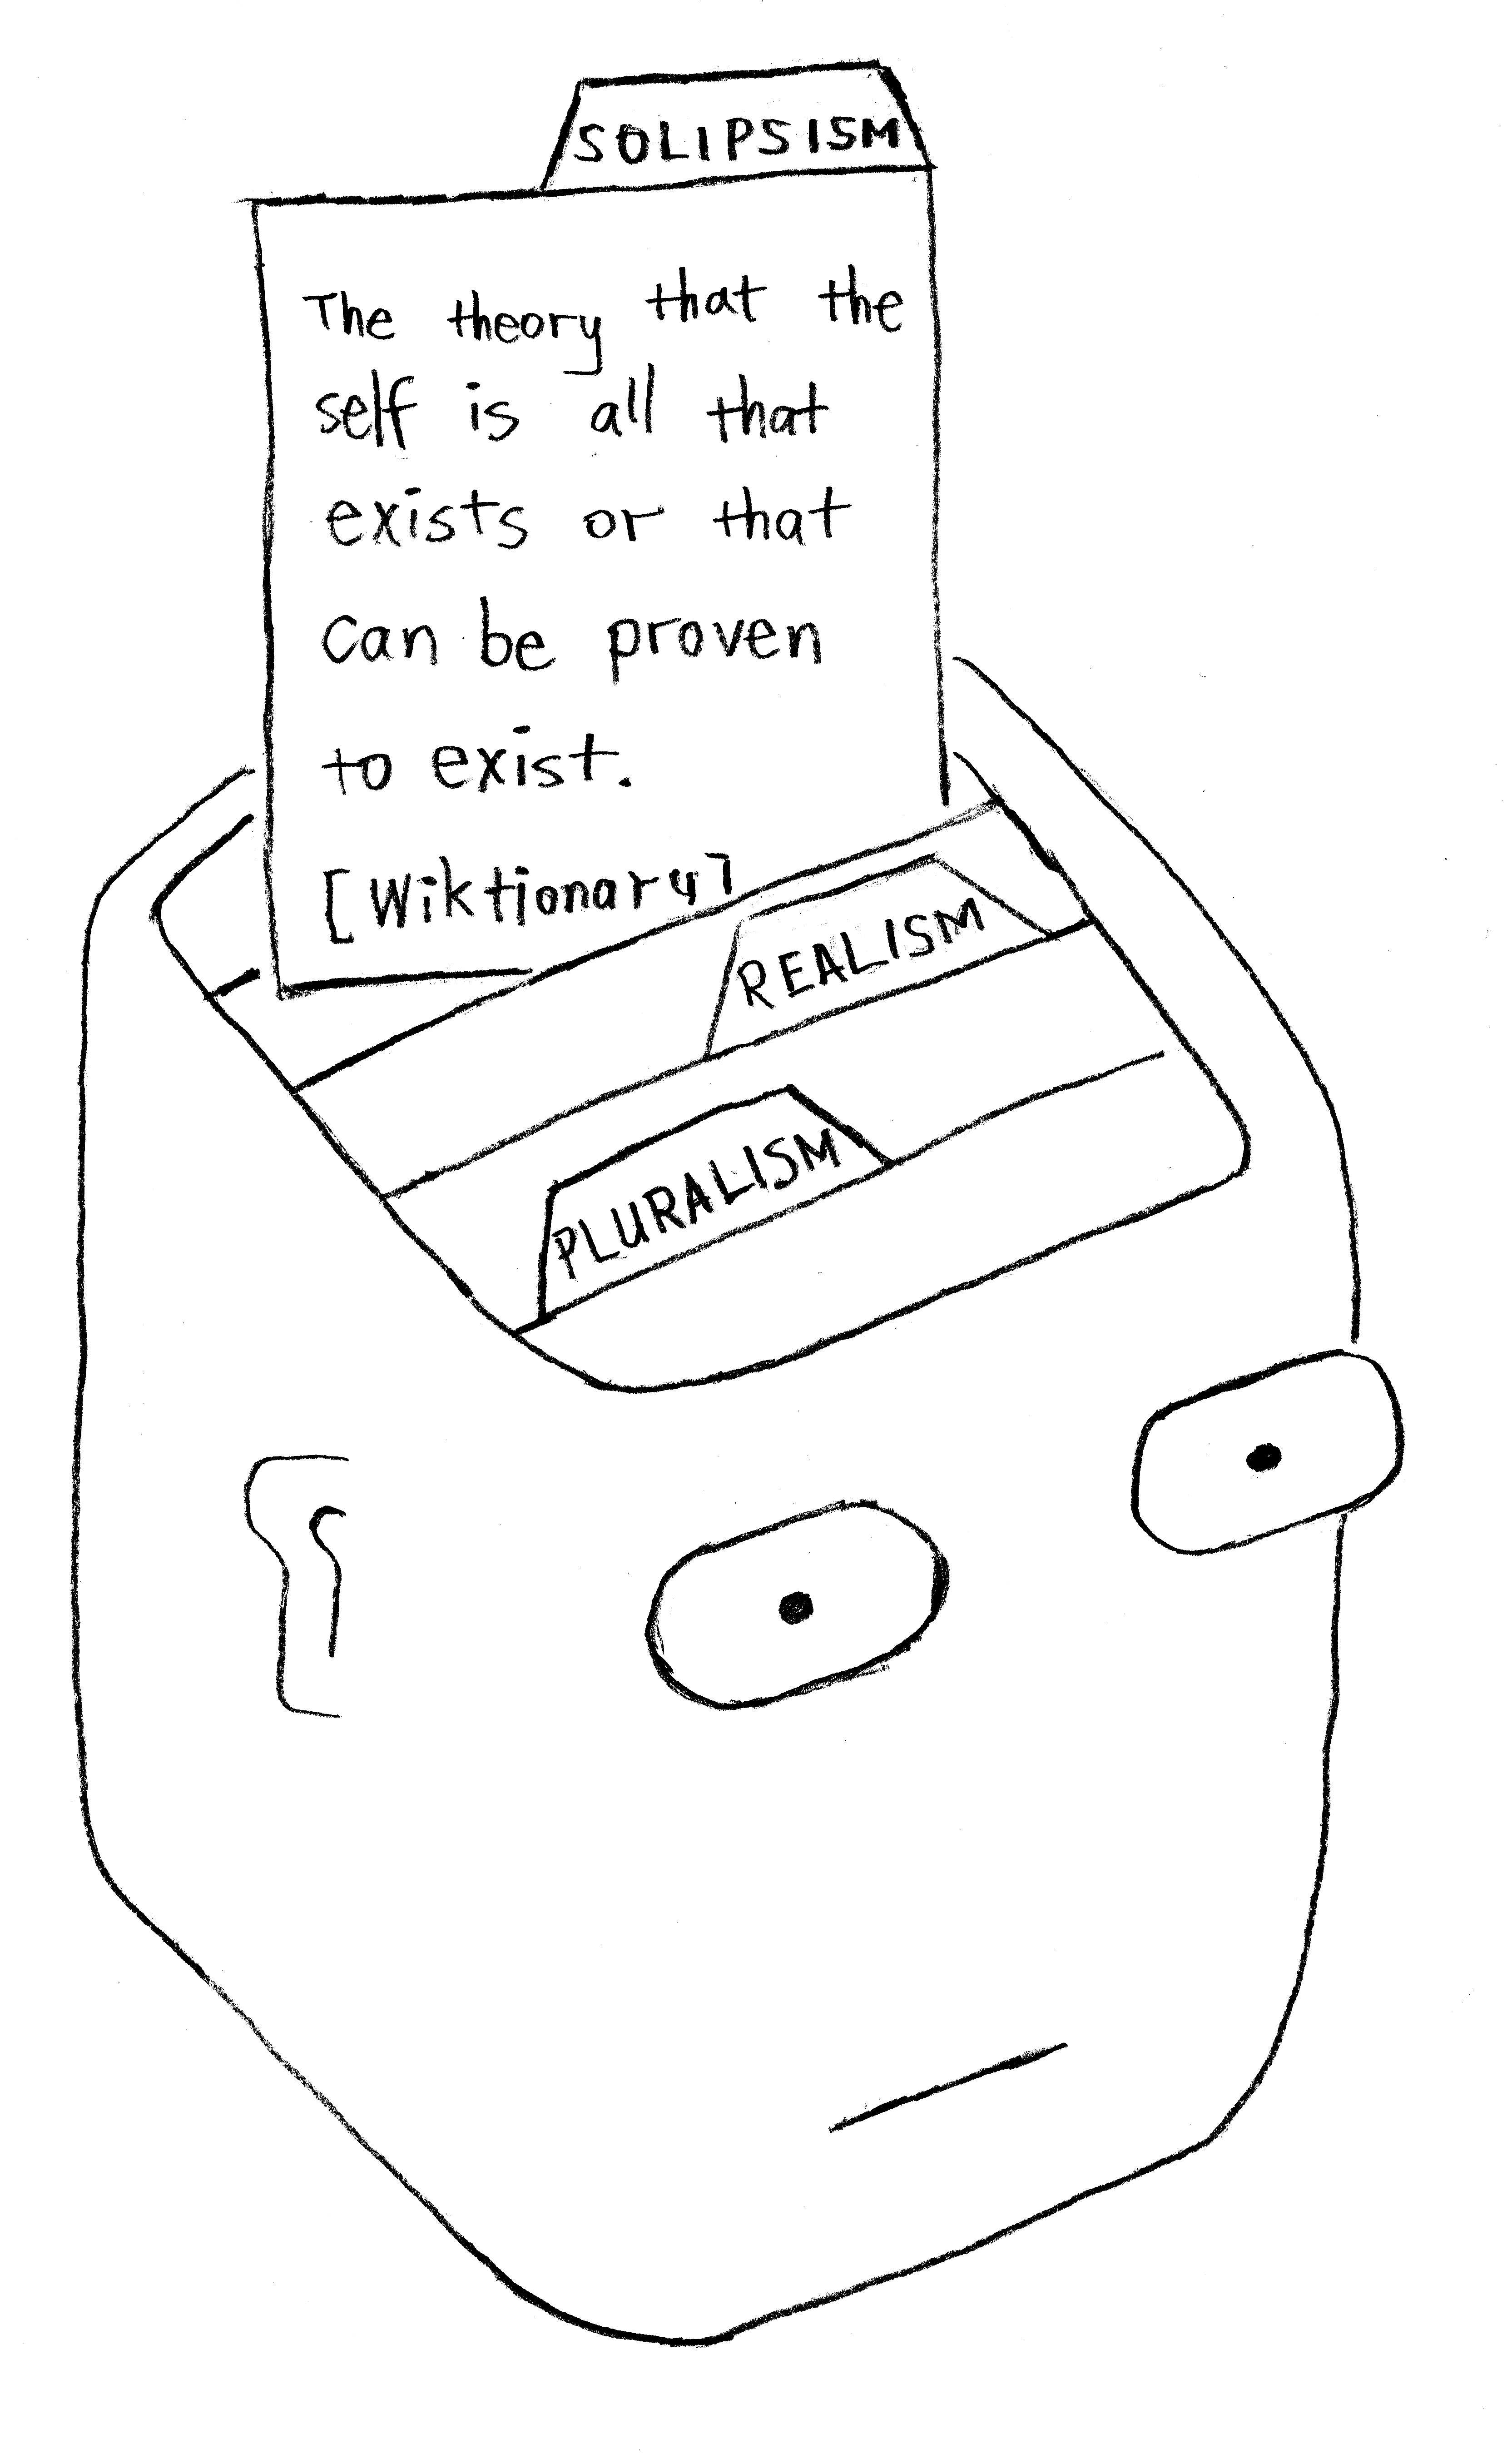
\includegraphics[width=21cm]{head.png}
\end{textblock}

% AUTHOR INFO
\begin{textblock}{20}(91,47.2)

\includegraphics[width=5cm]{Siegel_Uni_Marburg.png}
\end{textblock}
\begin{textblock}{14}(97,49.2)
Yufei Cai\\
Klaus Ostermann
\end{textblock}
\begin{textblock}{20}(91,53.2)
\FONTSIZE{28}
\url{cai@mathematik.uni-marburg.de}
\end{textblock}

% IDEAL MODEL
\begin{textblock}{20}(91,60.5)
\includegraphics[width=5cm]{ideal-model.eps}
\end{textblock}
\begin{textblock}{14}(97,60.5)
\CITE
%\vspace{1.5cm}
David MacQueen,\\
Gordon Plotkin,\\
Ravi Sethi.\\
\emph{An ideal model for recursive polymorphic types,} POPL~'84
\end{textblock}

% PLUGGABLE TYPES
\begin{textblock}{20}(91,69)
\includegraphics[width=5cm]{pluggable.eps}
\end{textblock}
\begin{textblock}{14}(97,69)
\CITE
%\vspace{1.5cm}
Gilad Bracha.\\
\emph{Pluggable type systems,} OOPSLA-RDL~'04
\end{textblock}

\end{document}
